\documentclass[12pt]{article}

\newcommand{\GroupId}{CC09-7}
\newcommand{\assignment}{project-usability}

\NeedsTeXFormat{LaTeX2e}
\usepackage[osf]{mathpazo}
\usepackage[svgnames]{xcolor}
\usepackage[T1]{fontenc}
\usepackage{amsmath,amsthm,amsfonts,amssymb,mathtools}
\usepackage{multicol}
\usepackage{float}
\usepackage[margin=2.7cm,a4paper]{geometry}
\usepackage{tasks}
\usepackage{xstring}
\usepackage[tikz]{mdframed}
\usepackage{environ}
\usepackage{subcaption}
\usepackage{etoolbox}
\usepackage{booktabs}
\usepackage{fourier-orns}
\usepackage{kvoptions}
\usepackage{units}
\usepackage{hyperref}
\usepackage{url}
\geometry{a4paper, margin=1in}
\usepackage{graphicx}
\usepackage{subcaption}


% math config

\DeclarePairedDelimiter\ceil{\lceil}{\rceil}
\DeclarePairedDelimiter\abs{\lvert}{\rvert}
\DeclarePairedDelimiter\set{\{}{\}}

% headers

\usepackage{fancyhdr}
\addtolength{\headheight}{2.5pt}
\pagestyle{fancy}
\fancyhead{} 
\fancyhead[L]{\sc info2222} 
\renewcommand{\headrulewidth}{0.75pt}

% update these headers
\fancyhead[C]{\sc Group Id: \GroupId}
\fancyhead[R]{Assignment \assignment}

\begin{document}

\section{User Investigation}

\subsection{Introduction}
\hspace{2em}In our project, we chose students as the target user group and conducted a survey through Ed and tutorial classes to gain a deeper understanding of their needs and preferences. The students who participated in the survey were mainly from computer science-related departments.

Through the survey, we found that students primarily use WeChat (55.1\%) and Instagram (24.5\%) to communicate with friends (61.2\%) and classmates (28.6\%). They like the user-friendly interface of these chat applications (71.4\%) and prefer the option to set multilingual support (54.5\%). Students hope that chat rooms will allow only the group owner to invite friends (63.3\%). Opinions were divided on whether new users should be able to see chat room history (55\% in favor, 45\% against). Based on these findings and lecture slides \cite{7.users-designs.pptx}, we conducted a PACT analysis for this group of computer science students and constructed relevant personas. The statistics for each question and the complete survey data are provided in the appendix (\ref{survey}).

\subsection{PACT Analysis}
\hspace{2em}\textbf{People:} (98\%) of respondents are students at the University of Sydney, with only one staff member participating. Students primarily use the platform for academic-related activities, such as discussions and posting questions. They also want to communicate with friends. Among the respondents, 55.1\% are currently using WeChat, and 24.5\% are using Instagram, indicating that a design similar to these apps would be more familiar to them. Most respondents are computer science majors, with a few students from other majors.

\textbf{Activities:} The platform's primary use cases include participating in discussions, sharing academic experiences, and asking questions. Additionally, the platform should support students in communicating with friends. In terms of functionality, 61.2\% of users primarily engage in group chats or private chats with friends, and 28.6\% chat with schoolmates. Users prefer that only group owners can invite friends to join group chats (63.3\%) and wish to retain chat history. Both staff and students can post articles and comment on them, with staff having the authority to manage posts and comments. Compared to other features, users highly prefer a friendly interface (71.4\%). Regarding additional features, 54.5\% of users want support for multiple languages.

\textbf{Contexts:} Considering the study and life of university students, they might use the platform both on and off-campus, including at home or during commutes. They can access the site anytime, with peak usage times during the day and evening. Teachers and staff need to be able to access the site at any time to manage student posts, requiring the platform to function reliably across different times and locations, providing a consistent user experience.

\textbf{Technologies:} Considering the usage patterns of university students, the platform must work on various devices, including laptops and phones. Given the diverse usage environments, the platform needs strong adaptive design to ensure a consistent and smooth user experience across all devices.

\subsection{Persona}
\textbf{Name:} Emma Zhang \\
\textbf{Age:} 20 \\
\textbf{Major:} Computer Science \\
\textbf{Background:} Emma is a second-year computer science student at the University of Sydney. She is proficient in using various technologies and spends a significant amount of time on her laptop and smartphone. She uses chat applications like WeChat and Instagram daily to keep in touch with her friends and classmates. \\
\textbf{Motivations:} 
\begin{itemize}
    \item Share experiences and ask questions related to her studies.
    \item Communicate with friends and classmates for both academic and personal purposes.
    \item Use a platform with a user-friendly interface and multilingual support.
\end{itemize}

\textbf{Frustrations:} 
\begin{itemize}
    \item Difficulty in finding a platform that combines academic and personal communication.
    \item Lack of multilingual support in many existing chat applications.
    \item Confusion caused by complicated interfaces in some chat platforms.
\end{itemize}

\textbf{Preferred Features:} 
\begin{itemize}
    \item User-friendly interface similar to WeChat and Instagram.
    \item Multilingual support.
    \item Ability for group owners to invite friends to join group chats.
    \item Retaining chat history for reference and context.
\end{itemize}

\newpage

\section{Navigation design}
\hspace{2em}We used Optimal Workshop for card sorting. As of 3:53 AM on May 16, a total of 11 participants completed the card sorting. The image is shown as figure \ref{cardsorting_overview}. We categorized the multilingual functionality, which we learned about from the previous survey, under the "User settings/profile" card, as this special feature pertains to the entire user interface settings. The similarity matrix of the results is shown in the figure \ref{similarity_matrix}.

\begin{figure}[H]
    \centering
    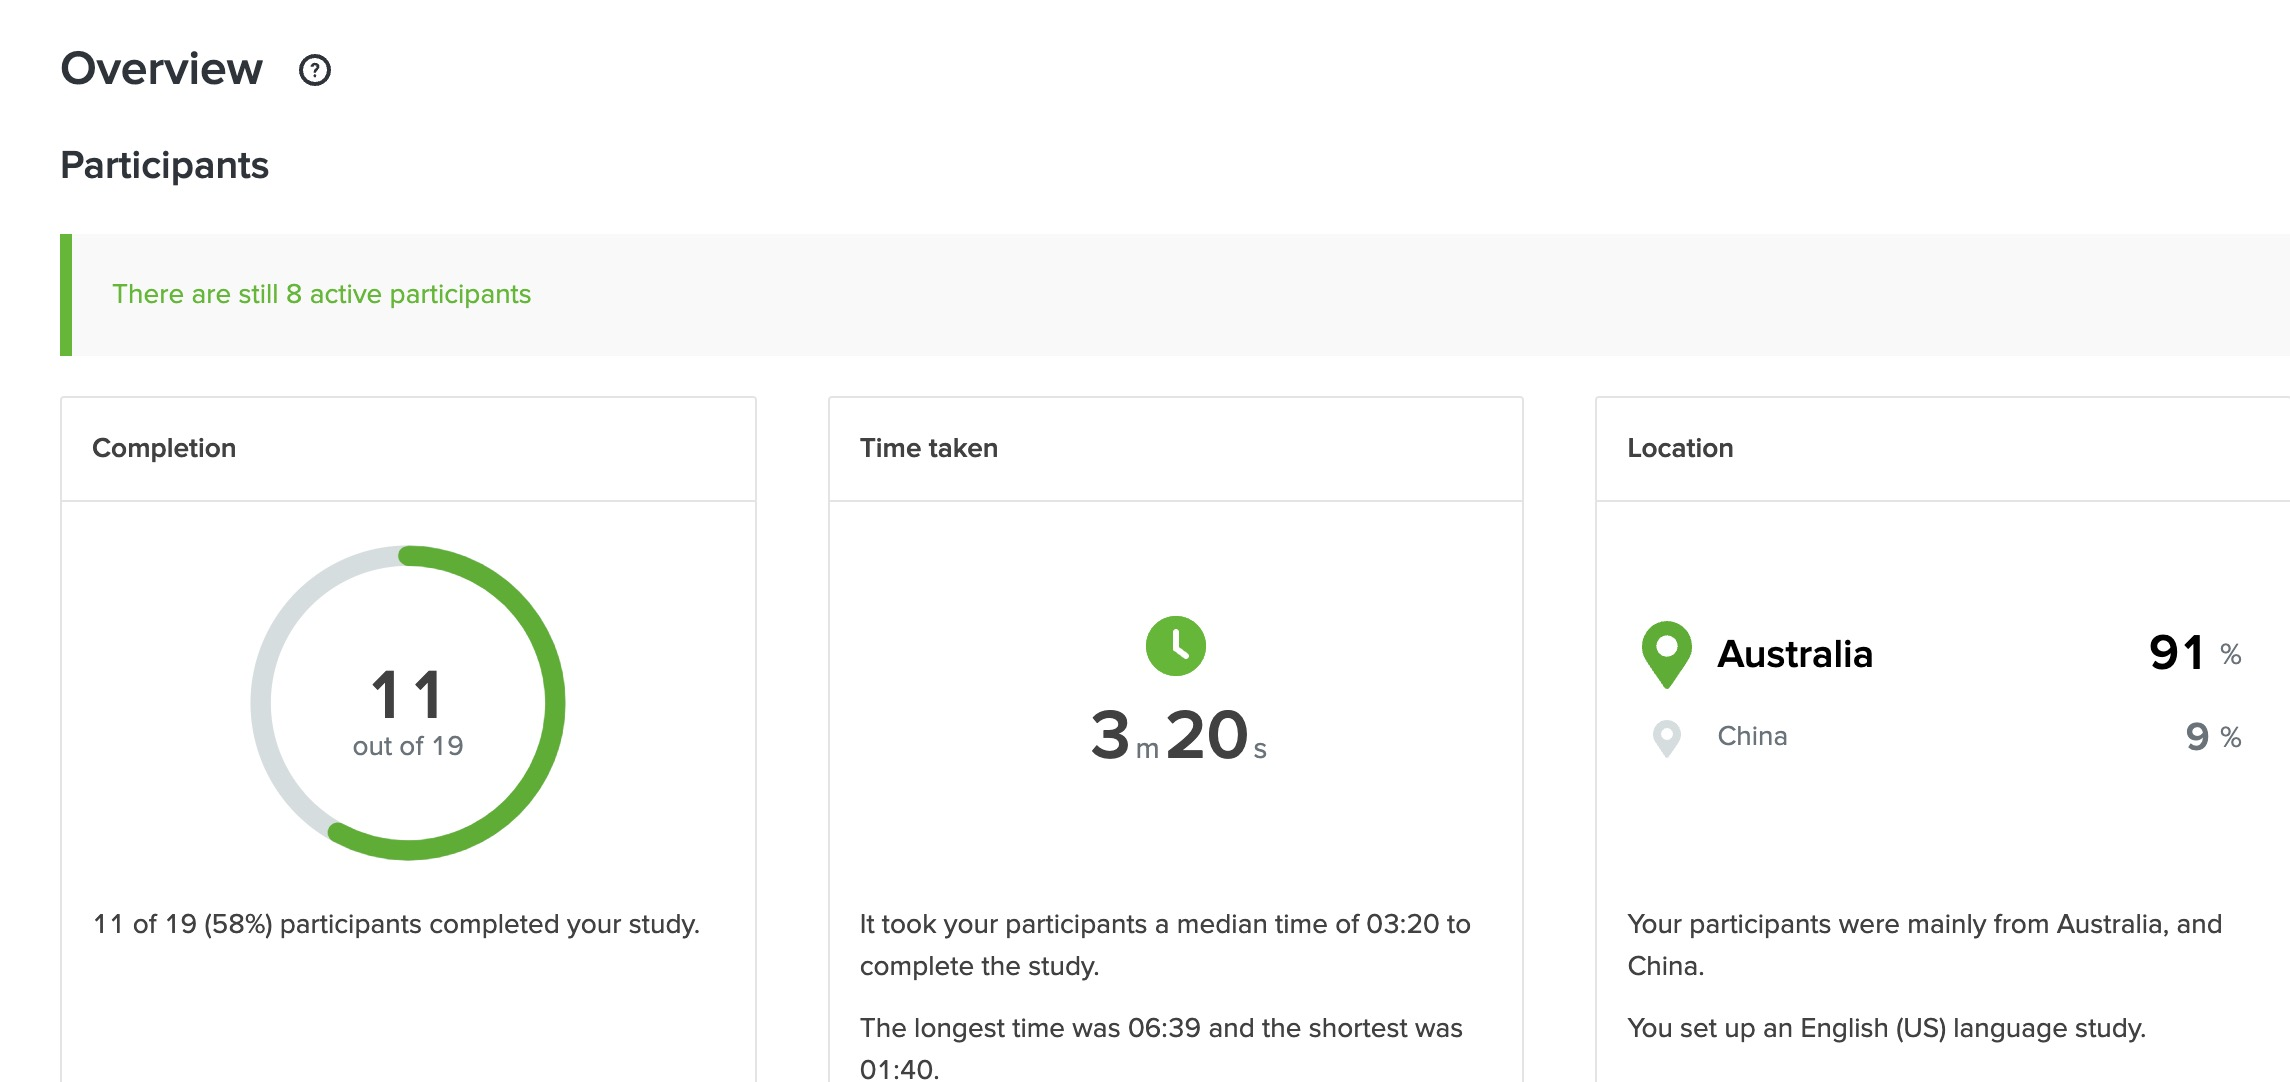
\includegraphics[width=0.9\textwidth]{graphs/cardsorting_overview.jpg}
    \caption{Card Sorting Overview}
    \label{cardsorting_overview}
\end{figure}

\begin{figure}[H]
    \centering
    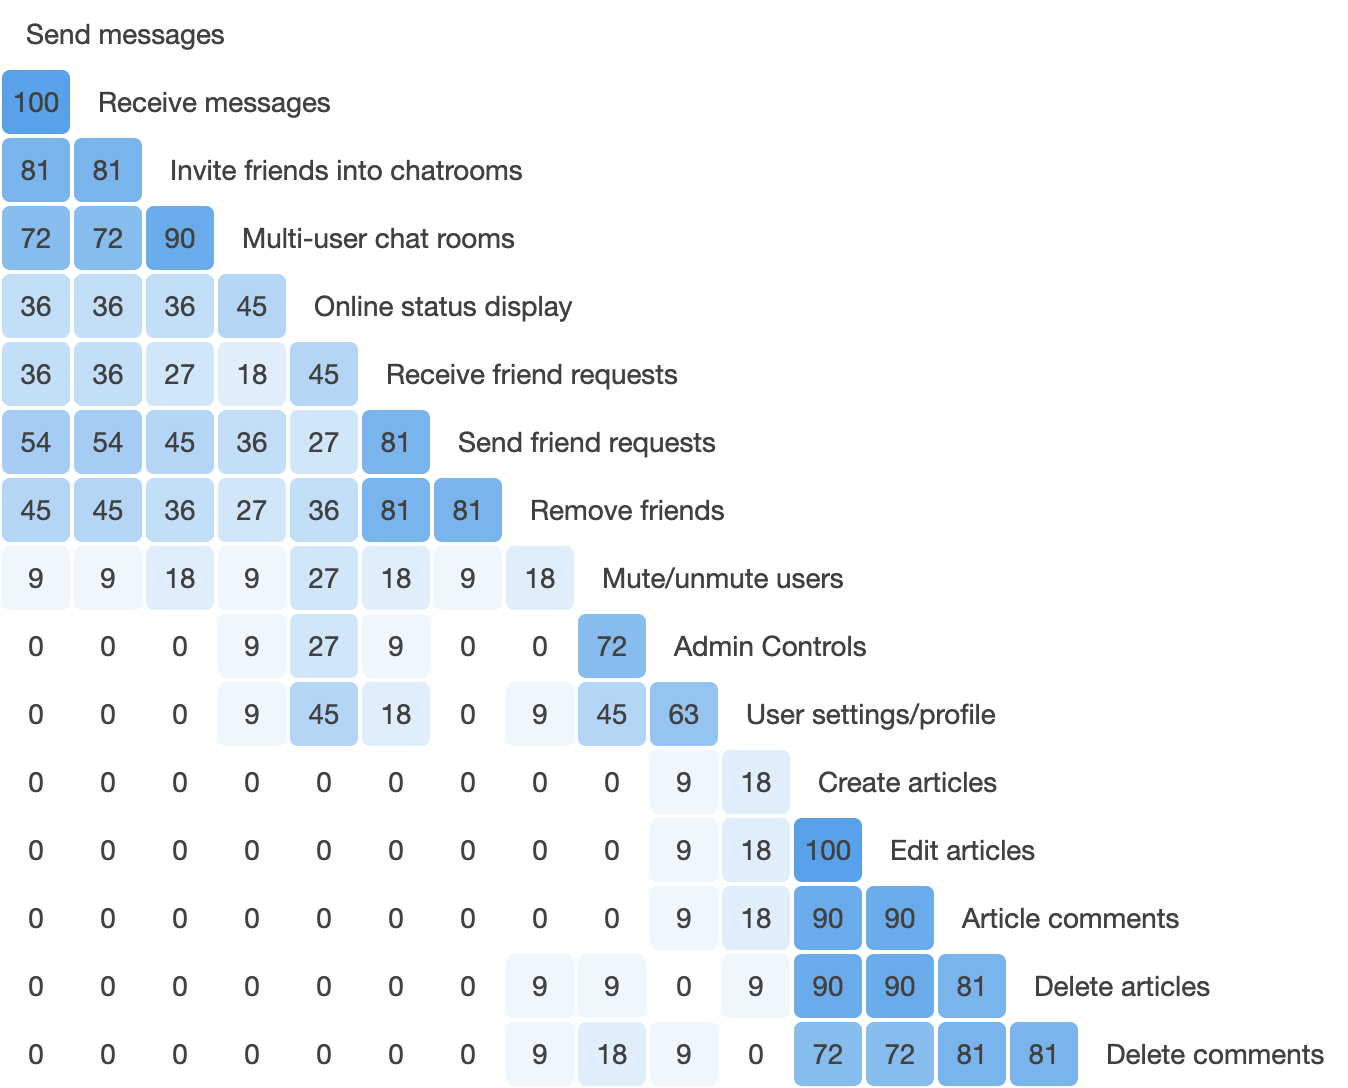
\includegraphics[width=0.8\textwidth]{graphs/Similarity_Matrix.png}
    \caption{Similarity Matrix}
    \label{similarity_matrix}
\end{figure}

\newpage

Based on the similarity matrix, we have categorized as follows:
\begin{multicols}{2}

\subsubsection*{Page: Messages App}
\begin{itemize}
    \item Multi-user chat room
    \item Send message
    \item Receive message
    \item Invite friend into Chatroom
    \item Online status display
    \item Receive friend requests
    \item Send friend request
    \item Remove friend
\end{itemize}

\subsubsection*{Page: Settings}
\begin{itemize}
    \item Admin control
    \item Mute/Unmute User
    \item User settings/profile
\end{itemize}

\columnbreak

\subsubsection*{Page: Knowledge Repo}
\begin{itemize}
    \item Create articles
    \item Delete articles
    \item Edit articles
    \item Article Comments
    \item Delete Articles
    \item Delete Comments
\end{itemize}

\end{multicols}

\section{Appendix}

    \subsection{User Investigation Survey Evidence}
    \label{survey}
        \textbf{Overview:}

        \begin{figure}[H]
            \centering
            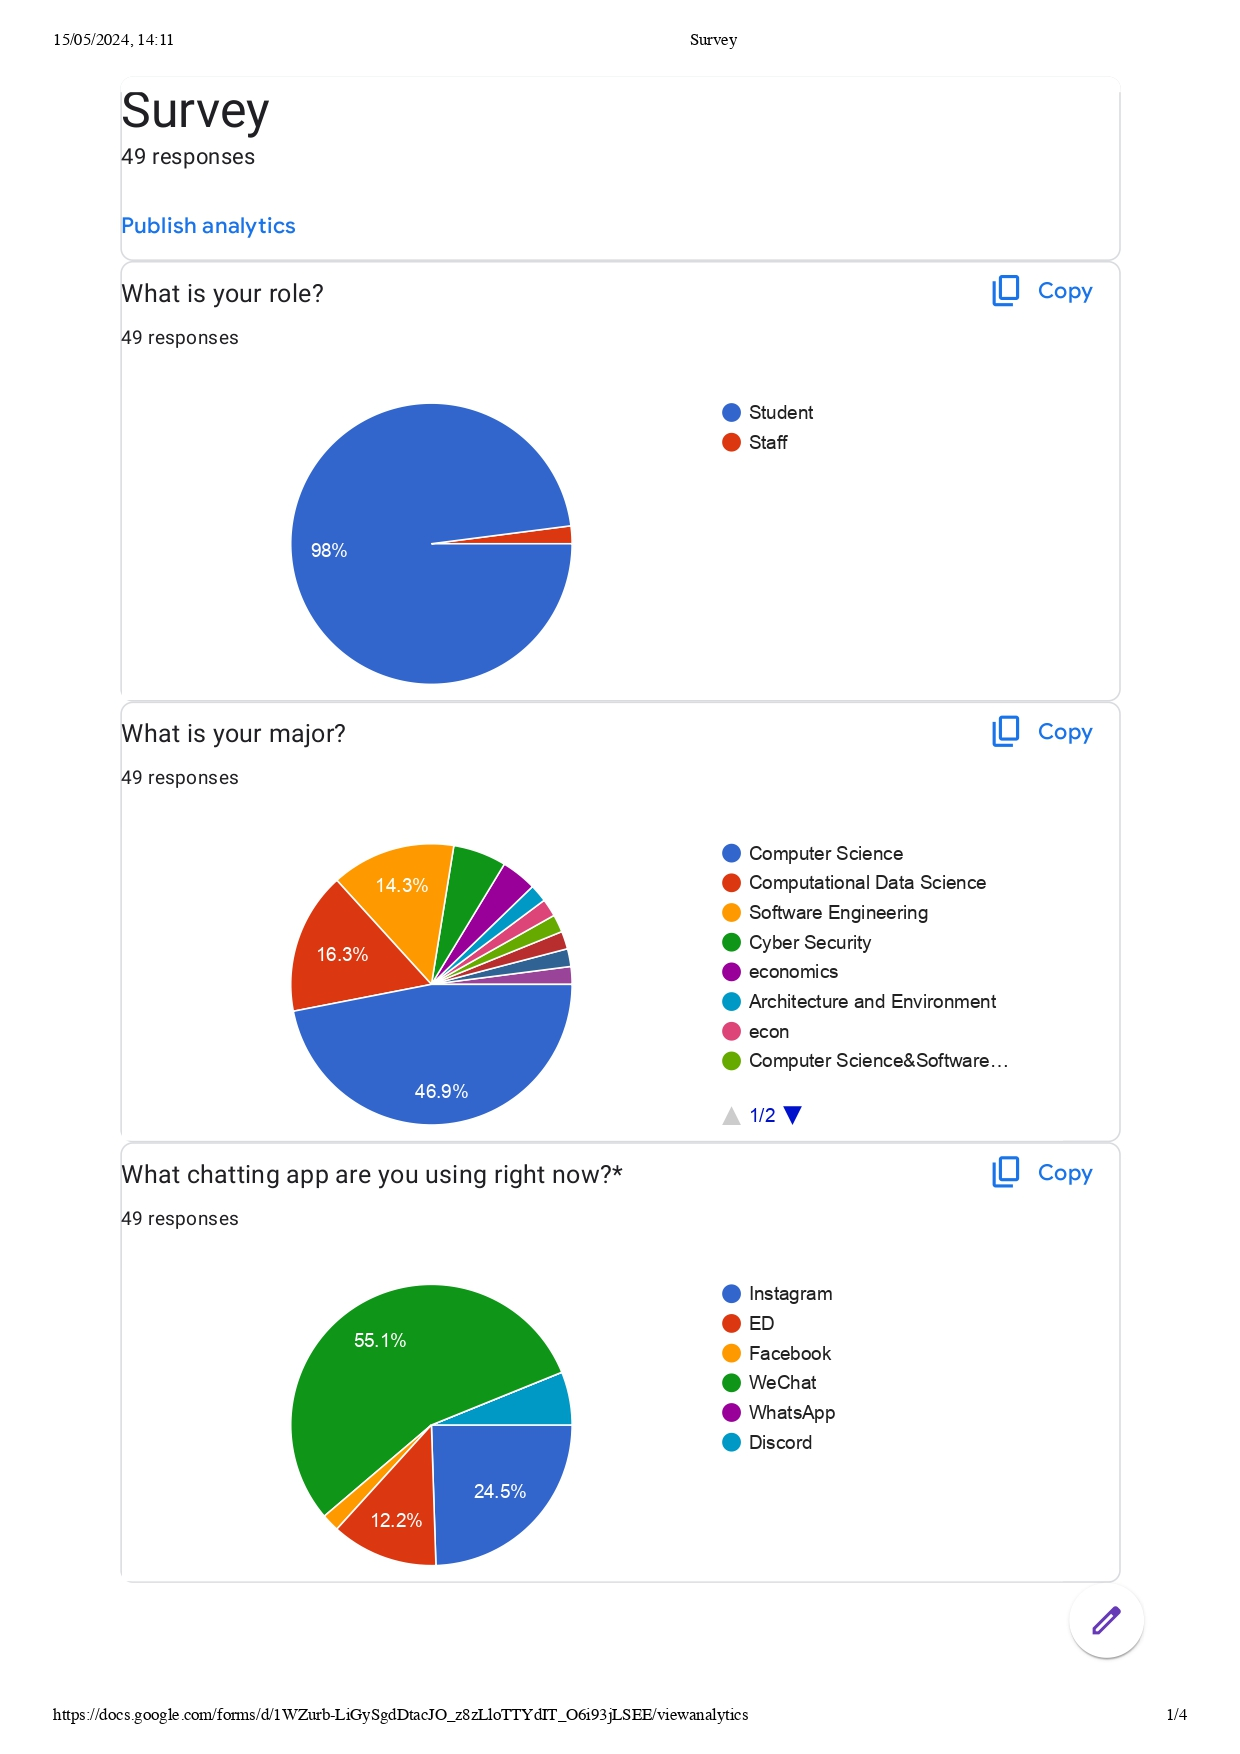
\includegraphics[width=0.9\textwidth]{graphs/Survey-summary_page-0001.jpg}
        \end{figure}

        \begin{figure}[H]
            \centering
            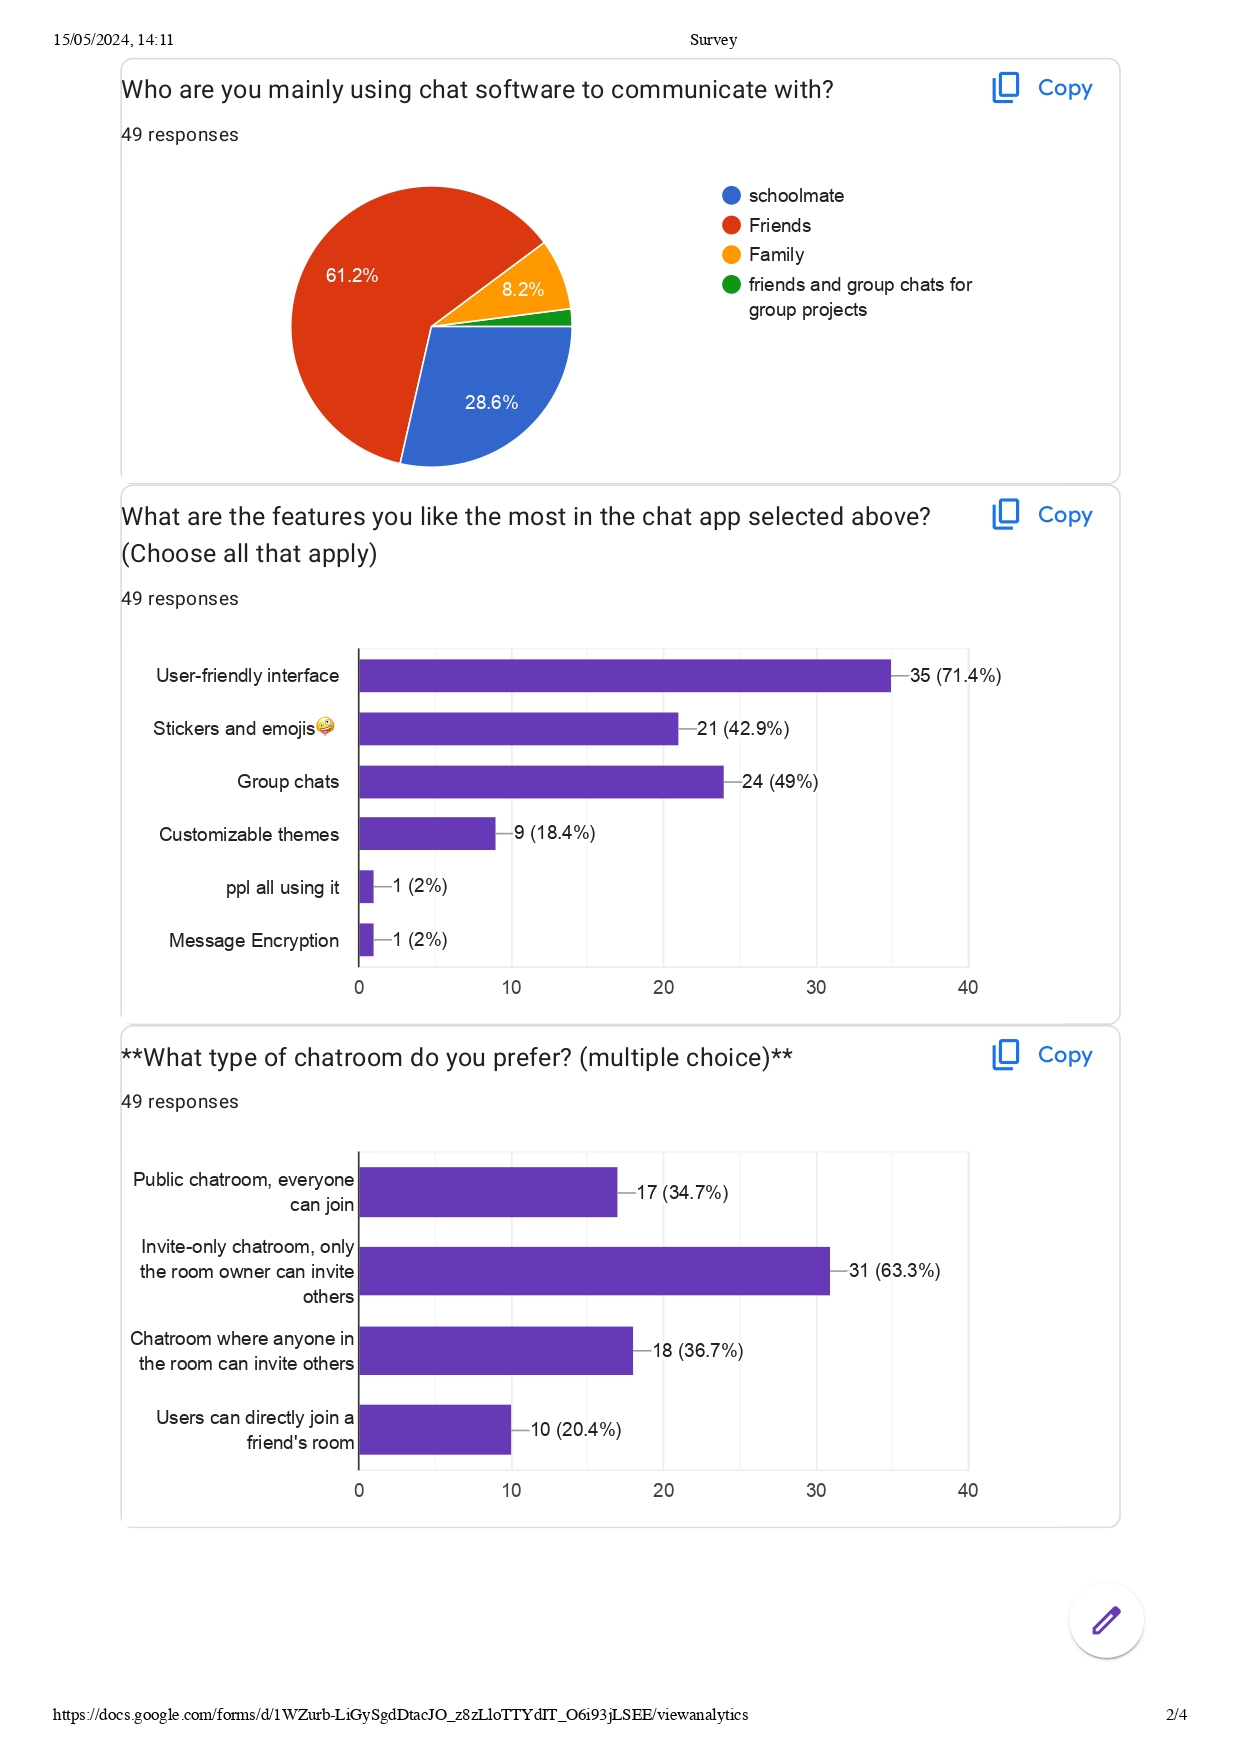
\includegraphics[width=0.9\textwidth]{graphs/Survey-summary_page-0002.jpg}
        \end{figure}

        \begin{figure}[H]
            \centering
            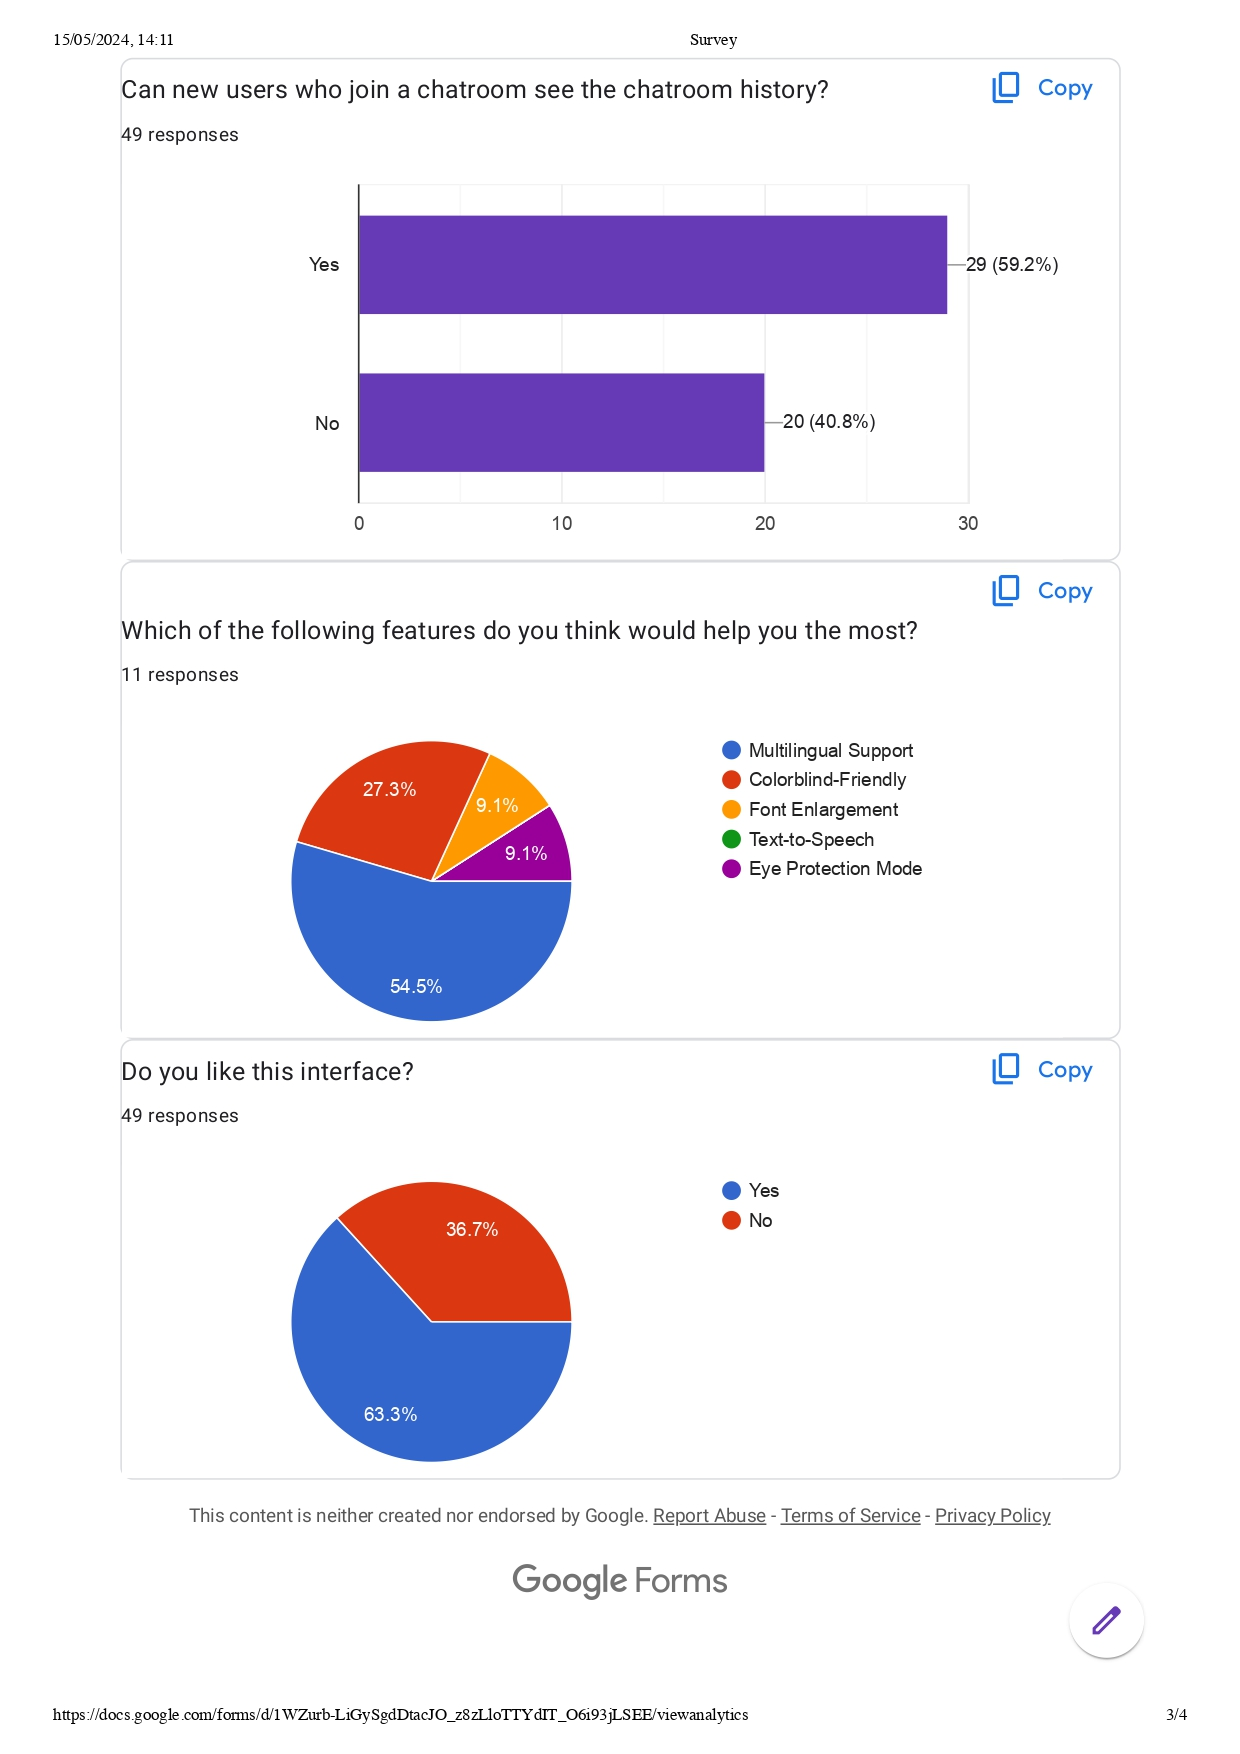
\includegraphics[width=0.9\textwidth]{graphs/Survey-summary_page-0003.jpg}
        \end{figure}

        \textbf{All Results}: /Evidence/Survey-all.pdf



\section{Design-Evaluate 1}



\section{Design-Evaluate 2}


\section{Contribution}

\bibliographystyle{unsrt}
\bibliography{reference} 
\end{document}
